%!TEX root = ../username.tex
\chapter{Neural Network} \label{chap:neural_network}

The group of Instance segmentation algorithms is a subgroup of object detection algorithms. All algorithms in the object detection group are required to do two tasks \cite{overview_cv_task}. 
\begin{enumerate}
    \item Generates a bounding box surrounding each object in the image.
    \item Classify the object in the bounding box.
\end{enumerate}
We first discuss the algorithm used for the classification task. Since in each bounding box, there is exactly one object to classify, an algorithm from the image classification task, a subset of the computer vision task, is applied \cite{overview_cv_task}.

% \hl{Conventional ML technique + limitation} \color{red} might put in the
% first para of NN section \color{black}
In the early day, as the first step toward artificial intelligence, a machine learning approach was proposed for the image classification task, but most were still designed manually by humans \cite{traditional_machine_learning}. Conventional machine learning uses feature extraction functions to map raw data to feature vectors. The feature vector is the only suitable data format that allows the learning subsystem of machine learning to detect patterns and classify the input. For that reason, the accuracy and effectiveness of machine learning methods are heavily dependent on the feature extraction function. However, the feature extraction function's responsibility is to extract features unique to the object that the machine tries to detect. Thus, the function requires an extremely detailed design and immense domain expertise to extract the feature of one object. Another disadvantage is that each object requires a different feature extraction function as they have unique features \cite{traditional_machine_learning}. The variety in features between objects causes the engineer to redesign the entire machine-learning architecture for each object which is a difficult task and inefficient.

% \hl{The paper outline}
As more studies go into the field, we start to move away from manually designed machine-learning methods to a more data-driven model. This data-driven algorithm group is now known as the artificial neural network.

% \hl{What is neural network}
Neural networks, also known as artificial neural networks (ANNs), are inspired by the human brain. Similar to the way the human brain processes and makes decisions, ANN is the core process of machine learning that gives the machine the ability to interpret the representation of raw binary data and move it toward artificial intelligence. An ANN algorithm is driven by data, the more data is supplied to the algorithm, the more accurate its interpretation ability becomes \cite{ai_data_driven}.

% \hl{Diff NN archietecture}
At the highest level of abstraction of ANN, there are two kinds of neural network architectures. The first and simplest one is feedforward architecture which allows its signal to travel from input to output \cite{lecun2015deep}. The feedforward network is widely utilized in grid patterns processing tasks, like image and video frames. The second architecture is the recurrent neural network (RNN). RNN expands the feedforward network's functionality by adding feedback connections that allow the network to feed its output back to the network \cite{lecun2015deep}. Feedback connections enable RNNs to be sufficient for processing sequences of data tasks.

% \hl{Hook to FC feedforward NN}
As this paper's interest lies in detecting objects of a scene, which require classifying individual objects in a grid of pixel values, we will only discuss the detail of a fully connected feedforward neural network.

\section{Feedforward Neural Network Architecture} \label{sec:feedforward_nn}

\begin{figure}[!ht]
    \centering
    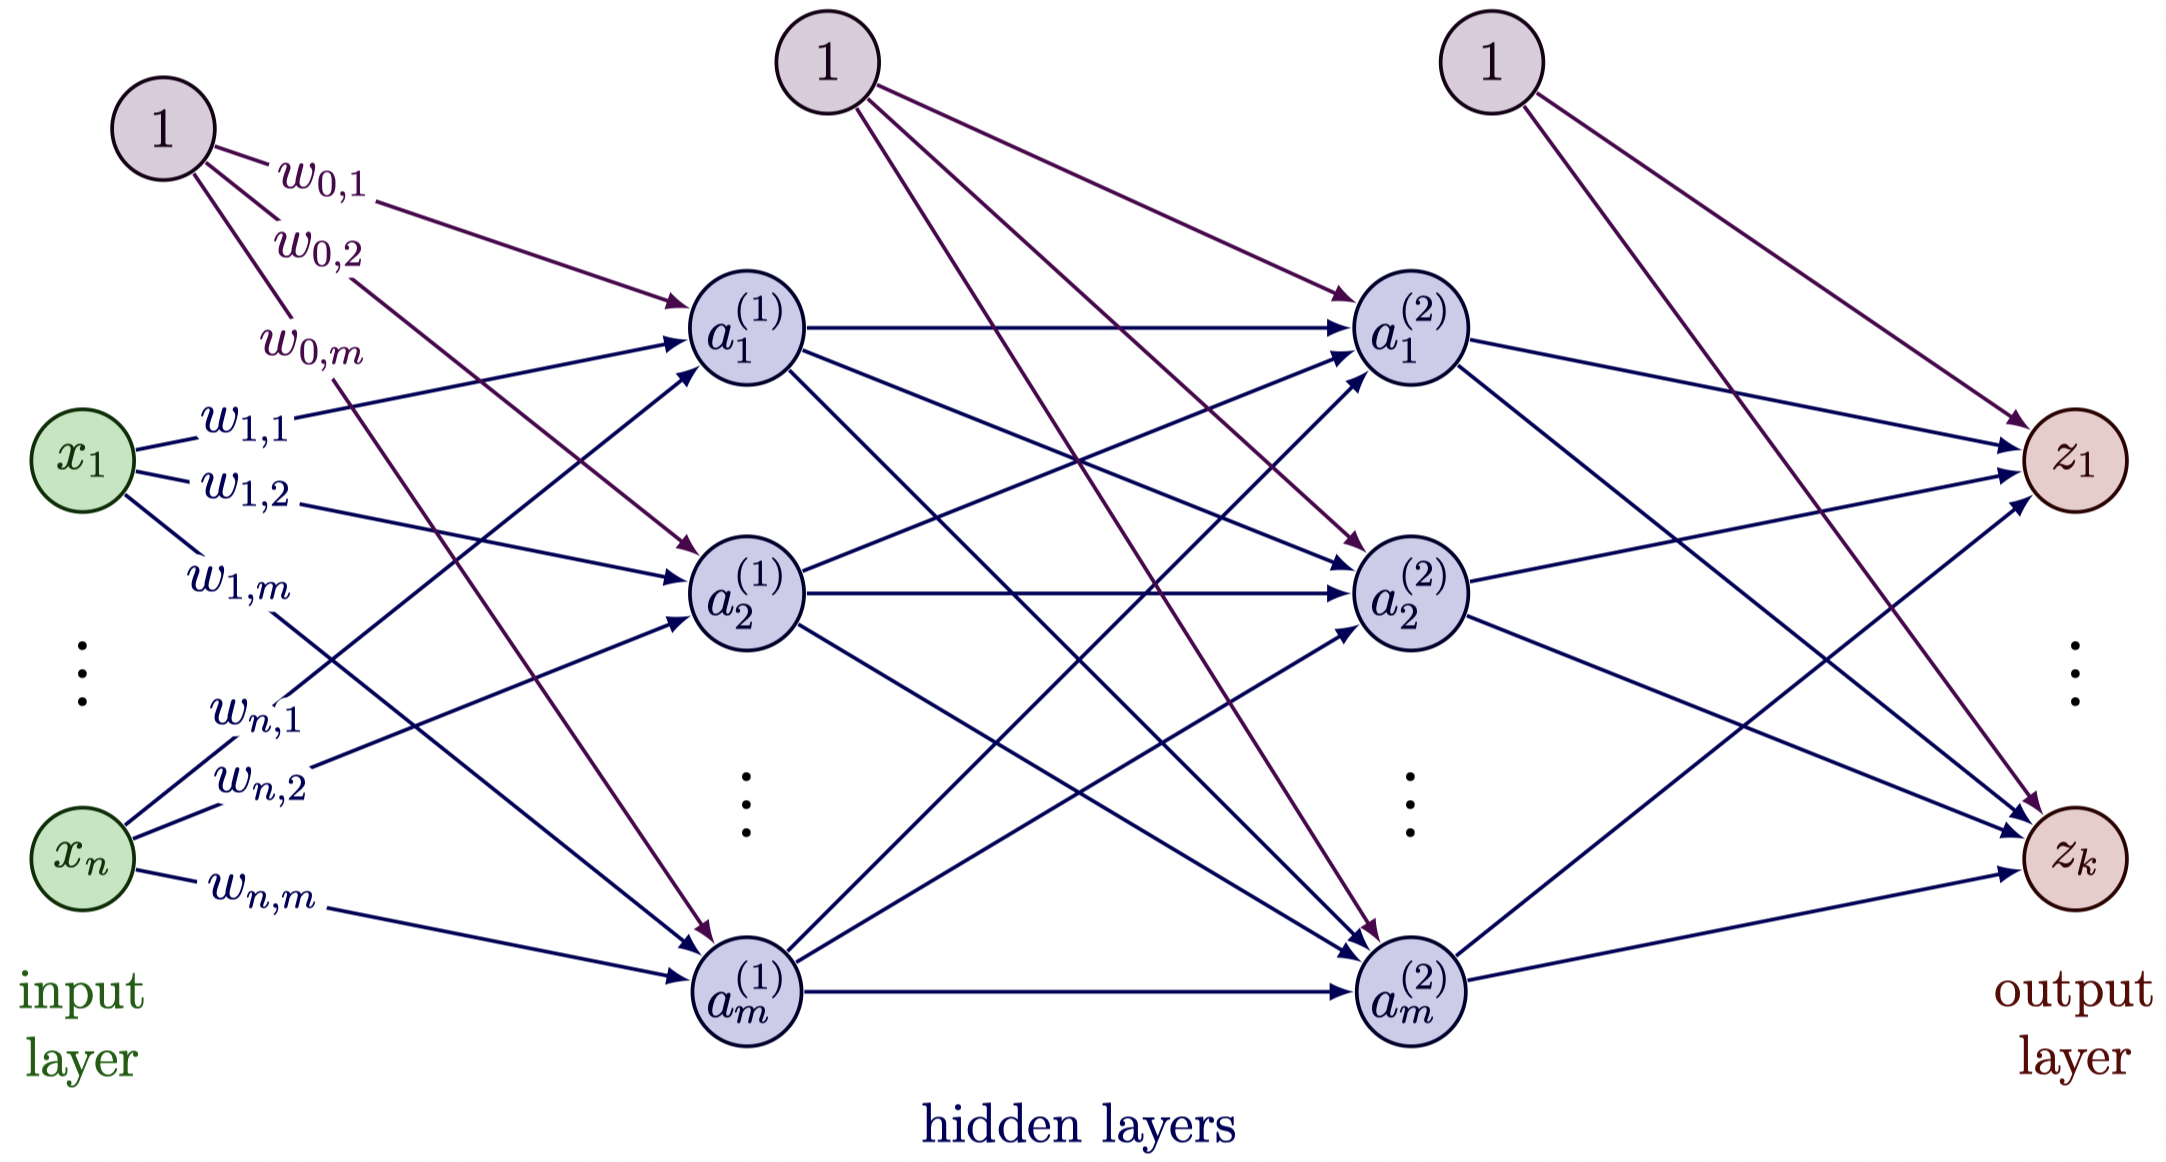
\includegraphics[width=5in]{figures/ffn_diagram.png}
    \caption{A Fully Connected Feedforward Neural Network} \label{fig:fc_ffn}
\end{figure}

Feedforward neural networks are the most basic type of deep learning model. Feedforward networks are designed to approximate a function that best maps the network's input to its output \cite{lecun2015deep}. On a high level, a feedforward neural network algorithm can be decomposed into four phases. The first phase is forward propagation, where the data flows through the network and initializes every node's values. The second phase is error evaluation, which determines how well the network does with its current setup. The third phase is gradient descent, where the algorithm determines which part of the network cause it to perform poorly. The last phase is backpropagation, where the algorithm updates the internal part of the network to make it more accurate and better fit the input data set. These four phases are applied and repeated on an extensive data set to become more precise over time. We will discuss more about each phase of the algorithm in this section, but we first need to understand the basic structure of a feedforward neural network.

\subsection{The Network Structure \label{network_structure}}
% \hl{Network layer}
To understand the feedforward network structure, we first need to define the idea of layers in the context of ANN. A \textbf{layer} in a neural network is a collection of neuron nodes at a specific network depth. A layer is represented by a column of node in Figure \ref{fig:fc_ffn}. A feedforward network can be thought of as a stack of multiple layers. Each layer in the stack is responsible for transforming the layer's input to help make sense part of the representation for later layers. On a high level, the network consists of the \textbf{input layer}, single or multiple \textbf{hidden layers}, and the \textbf{output layer}. The number of hidden and output layers is the \textbf{depth} of the network. As an example, Figure \ref{fig:fc_ffn} is a fully connected feedforward neural network with a depth of three.

% \hl{Network neuron + activation signal}
Each layer consist of one or more nodes. Each node in a layer represents an \textbf{artificial neuron}. The number of neurons in each layer can be different from one another. Each neuron holds a numerical value called the \textbf{activation signal}. In theory, the activation signal takes on any value in the real numbers set $\mathbb{R}$. However, in practice, studies have shown multiple advantages, {\color{red} like improved training time and avoiding overfitting problems [section 2.3]}, when normalizing the activation signal of every neuron \cite{lecun2012efficient}. As an example, we consider a network that receives a $23 \times 23$ RGB image and then produces a dog or cat label for the object in the image. In the input layer, the number of neurons is the total pixel in the image in each color channel, that is $23 \times 23 \times 3$ neurons, and each neuron (denoted $x_i$) holds that pixel value normalized. On the other hand, the output layer only has two neurons (denoted $z_i$); one corresponds with the dog and the other with the cat. Unlike the input and output layer, where the number of neurons needed is straightforward, the number of neurons in each hidden layer and the number of hidden layers are complicated to determine and remain outside the scope of this paper. However, studies have shown that networks with the same neurons' hidden layers perform better \cite{taylor2017neural}, and deeper networks result in more advanced learning with some issues like gradient vanishing and more {\color{red} [section 2.3]}. {\color{red} Discuss overfiting and gradient vanishing problem in section 2.3}

% \hl{Network connection + weight}
Each neuron in a layer can affect a neuron from the next layer through a \textbf{connection}. The connection is represented by a line between two neurons in Figure \ref{fig:fc_ffn}. In fully connected networks, each neuron in a layer will be affected by all the neurons from the previous layer. In other words, each neuron will have a connection with every neuron in the previous and next layer of the network. Associate with each connection is a numerical value representing the \textbf{weight}. The weight of a neuron infers how influence the neuron will be on the next layer of the neural network. A small weight value means the activation signal of this neuron has a low effect on neurons of the next layer. On the other hand, a high weight value results in a more significant effect proposed by this neuron to the next layer and the network's output. When a neural network algorithm initialize, its weights are randomly assigned using a Gaussian or uniform distribution \cite{lecun2015deep}. {\color{red} Discuss Gaussian or uniform distribution in section 2.3} These weights are adjusted as the neural network algorithm process to best approximate its mapping function. The weight from neuron $a_i$ to a neuron $a_j$ in the next layer will be denoted as $w_{i,j}$ with the exception of bias's weight.

% \hl{Network bias}
In addition to the weight, neurons in each layer other than the input layer are also influenced by a \textbf{bias node}. A bias node is represented by a node that always holds value 1. The bias node has connections to every neuron in the layer it affects. Each bias's connection also has a weight associated with it. The connection between bias and neuron $a_j$ in the affected layer will have its weight denoted as $w_{0,j}$. The role of the bias node is like a threshold to the neuron. In other words, the bias determines how significant the activation signal of a neuron must be before that neuron gets propagated to the next layer of the network. Similar to weight, when the network initializes, the bias's weight is randomly assigned a value, and this value is optimized as the algorithm process. In the forward process of the network, the algorithm will compute a net input that requires a multiplication between a neuron activation signal and its weight. Since the bias node always has an activation signal of 1, thus the bias weight is the variable that directly affects nodes in the next layer. Therefore, the bias's weight is often refers as the bias.

These basic building blocks create the internal structure of a feedforward neural network. Some internal parts are also known as internal variables or network parameters. The model parameters refer to variables that are learnable in the gradient descent process, and they are not set manually by the developers. Weights and bias weights are examples of the network's parameters. In contrast with parameters, hyperparameter refers to variables manually set by the developers and sometimes can be optimized through training. Examples of hyperparameters are the learning rate and batch size, which we will touch on more in the gradient descent section.

% \hl{Hook to forward propagation}
With the basic structure of the fully connected feedforward neural network in mind, we will discuss the first phase of an ANN algorithm. That phase is forward propagation.

\subsection{Forward Propagation} \label{forwardprop_section}
Forward propagation refers to the process by which the data move from the input layer to the output layer of the network. Regarding the image classification problem, the forward propagation process moves a list of raw pixel values through the network and gives out a number for each class label. These numbers are the \textbf{network's raw ouput}, and each number represents how likely the image is a member of this class. The forward propagation process uses two functions to evaluate the activation signal of each neuron in hidden and output layers. These two function are the \textbf{summation function} and the \textbf{activation function} \cite{taylor2017neural}.

\begin{wrapfigure}{l}{2.5in}
    \centering
    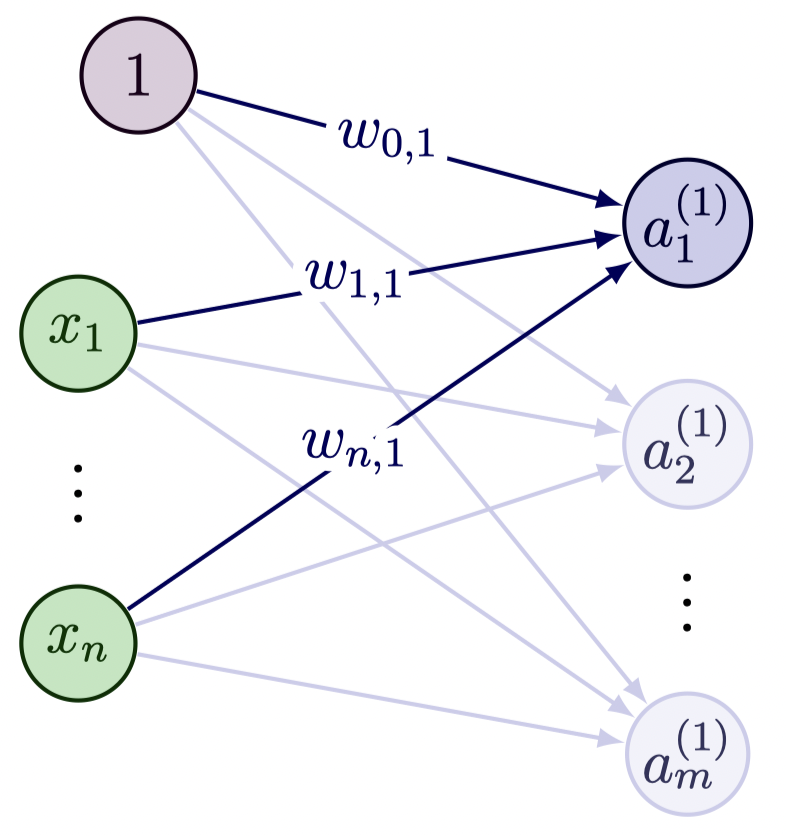
\includegraphics[width=2in]{figures/fp_diagram.png}
\end{wrapfigure}

% \hl{Summation function}
\noindent In a fully connected network, the summation function combines all neurons and their weight from the previous layer to create the net input for the current neuron. In general, the summation function can be expressed as \[net\ input\ of\ a_j = \sum_{i=1}^n (x_i w_{i,j}) + 1 \cdot w_{0,j}\] where $a_j$ represents the neuron that has the summation function compute its net input. The neuron's net input will then be transformed by an activation function.

% \hl{Activation func}
The activation function is responsible for transforming the net input into an activation signal, indicating if this neuron will affect later network layers. Additionally, linear functions are closed under addition, that is, adding or subtracting multiple linear functions from or to another function will result in a linear function. This fact implied that the feedforward network must have non-linearity terms if it approximates a non-linear function. The use of the activation function enables the network to introduce non-linearity terms to the algorithm. Furthermore, studies have shown that the output of a network - a network that only uses a linear activation function or does not use an activation function - will be a linear combination of its input, which means hidden layers have no effect \cite{He_2015_ICCV}.

% \hl{Most common activation function} 
There are numerous activation functions proposed, each with different strengths and weaknesses. However, in practice, there are four functions and their variance that are widely used by the ANN algorithm. These four activation functions are the linear, sigmoid, hyperbolic tangent (tanh), and rectified linear unit (ReLU). The formula and graphical representation of each function are shown in Table \ref{acti_func_table}.

\begin{figure}[!ht]
    \centering
    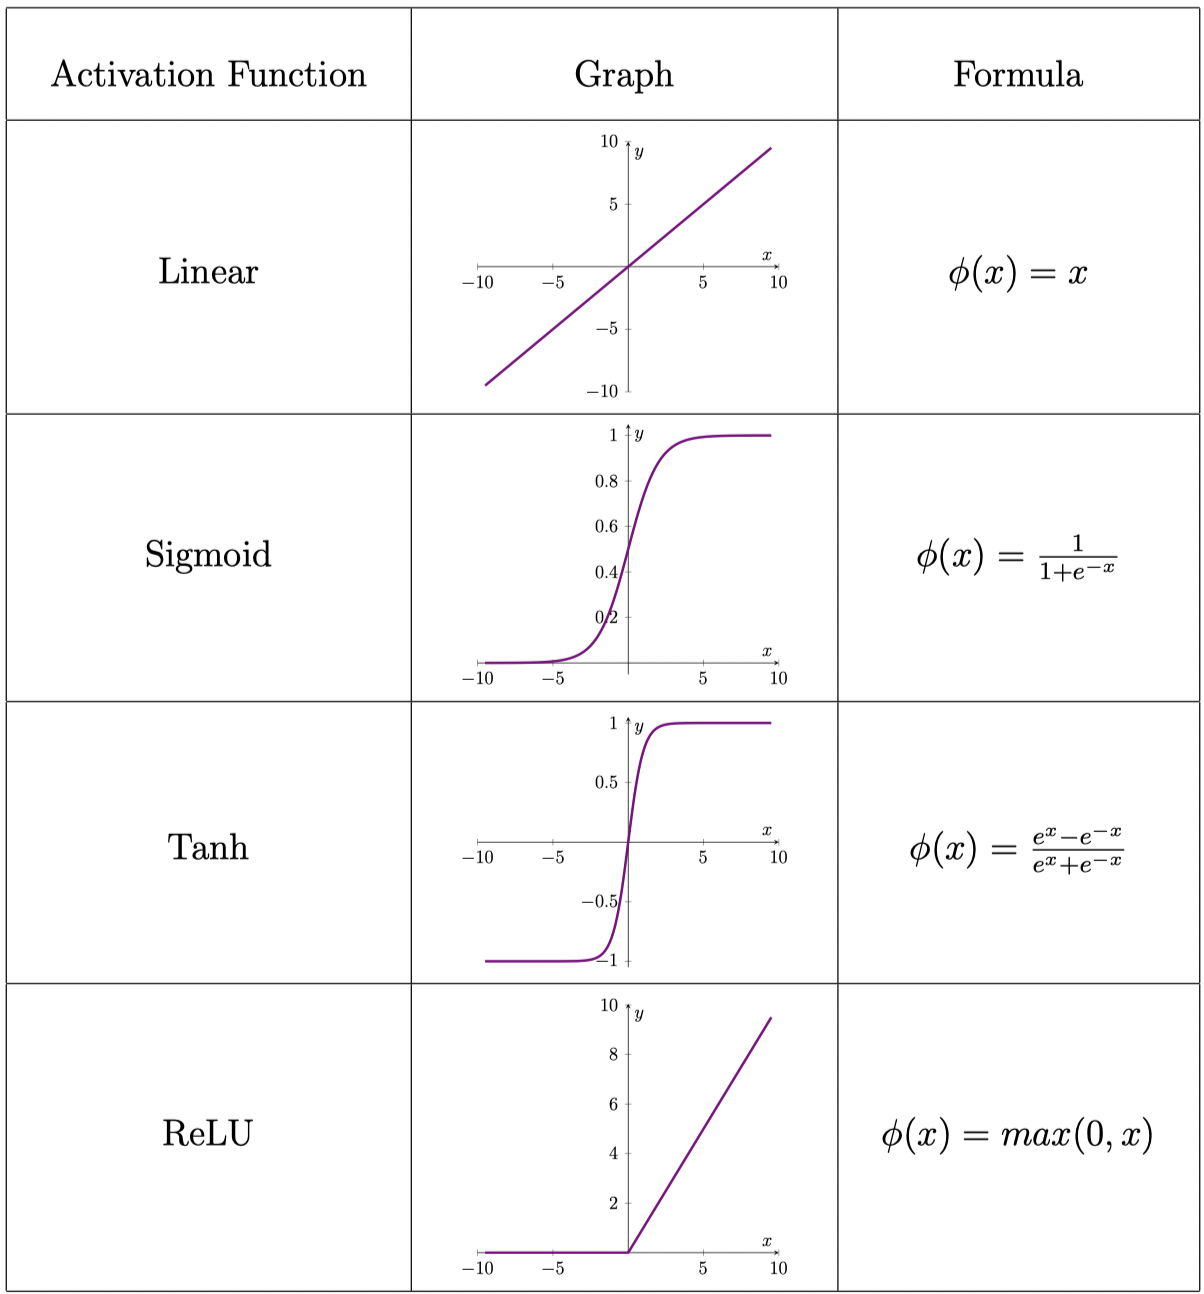
\includegraphics[width=5in]{figures/acti_func_table.png}
    \caption{Most Common Activation Function}
    \label{acti_func_table}
\end{figure}

% \hl{Activation func strength + weakness - need rewrite?} 
To understand which activation function to choose for a network, we need to know some important strengths and weaknesses of each function. First of all, the linear function is simple; thus, it forgiving and undemanding about the resources required for training. However, the linear function is close under addition; thus, the network will only be able to approximate a linear mapping function. In contrast, sigmoid and tanh are non-linear functions, thus allowing the network to approximate a non-linear mapping function. Additionally, sigmoid and tanh map real number set to (0, 1) and (-1, 1), respectively. The mapping of sigmoid and tanh allow the activation signal to be normalized, thus improving training time and avoiding exploding gradients \cite{lecun2015deep} {\color{red} [section 2.3]}. However, the mapping also causes sigmoid and tanh to suffer from the vanishing gradients problems. Different from sigmoid and tanh, ReLU map positive signal to itself, thus able to avoid the vanishing gradients problems. The first disadvantage of ReLU is it does not have any upper bound, which require the network to have some additional nomalization layer like batch normalzation (BN), weight normalizaiton (WN), and layer normalizaiton (LN) to optimize the training process \cite{relu_optimization_2020} {\color{red} [section 2.3]}. The second disadvantage of ReLU is it suffer from the dying ReLU problem which cause by the fact that all negative signal is map to 0 {\color{red} [section 2.3]}. Despite the dying ReLU problem, ReLU proves to be very efficient and accurate in practice; thus, it is the most used activation function currently \cite{li2021survey}. Furthermore, some variance of ReLU has been proposed to avoid the dying ReLU problem like Leaky ReLU and ELU. The problems possessed by these activation function is crucial when it comes to choosing an activation function and can be read more at LeCun et al., \cite{lecun2015deep}.

\subsection{Error Evaluation}
Once the forward propagation is completed, the algorithm will need to determine the correctness of the network with the current weight and bias. In order to estimate the network's correctness, the algorithm computes the difference between the network's output and the expected output. This process is known as the \textbf{error evaluation phase}, and it uses a \textbf{loss function} to quantify the difference. The three most used loss functions are \textbf{Mean Absolute Error} (MAE), \textbf{Mean Square Error} (MSE), and \textbf{Cross-Entropy}. MAE and MSE are primarily used in regression problems, while Cross-Entropy is mainly used in classification problems \cite{li2021survey}. As the focus of this paper is on the image classification task, we will only focus on Cross-Entropy.

Cross-Entropy is a loss function that is always used in conjunction with a softmax layer. A \textbf{softmax layer} is a layer that has the same number of nodes as the network's output layer. The goal of a softmax layer is to transform the raw output into probabilities for classes in the network's output, denoted $\hat{y}$. In other words, each neuron node activation signal is a class's probability after the softmax layer and is bounded by 0 and 1; and the probabilities of all classes must add to 1. The softmax layer use a softmax function to map a raw output value to the range $0-1$. The \textbf{softmax function} is defined as follow:
\[
    \hat{y_i} = \sigma(z_i)=\frac{e^{z_i}}{\sum^k_{j=1}e^{z_j}} \text{ \qquad
    with } i = 1, 2, 3, ... , k
\] 
where $z_1, z_2, z_3, ... , z_k$ are the value of network's raw output. The use of a softmax layer is crucial for output interpretation. Since a raw output does not have a lower or an upper bound for its value, thus different image might result in a different value range for the class label. This wide range of value behavior makes the raw output extremely hard to interpret and compare with the output of other images. The softmax layer standardizes the output by mapping the raw output to the range $0-1$ before comparing and calculating the error.

% \hl{cross-entropy loss} 
The softmax layer enables us to represent the network's output as a probability distribution for the object's class with a higher value means the object is more likely to be a member of that class. Similarly, we can also represent our desired classification output as a probability distribution with 1 for the object's class and 0 for all other classes. With that in mind, we have the Cross-Entropy function able to quantify the difference between two probability distributions, thus we use it to determine how far the network's output is from the actual desired output. The Cross-Entropy value of a standardized output neuron can be computed as follow: \[\text{CE of }\hat{y}_i = -\sum^k_{i=1} t_i \times \log(\hat{y}_i)\] where $t_i$ is the expected class$_i$'s value for the object present in our input image and $\hat{y}_i$ is the class$_i$'s probability for the object predicted by the network.

The Cross-Entropy for a neuron above describes the distance between the neuron's current activation signal and its expected value. By computing the Cross-Entropy for every output neurons, the sum of these Cross-Entropy values gives us the total error of the network. That is, the total Cross-Entropy describes how far the network is from its expected output in a single value and can be formularized as follow:
\[
    \text{Total Cross-Entropy} = \sum^k_{i=1} \text{Cross-Entropy of }\hat{y}_i
\]
where $k$ is the number of output neurons i.e. the number of class that we are trying to classify. Since total Cross-Entropy gives us a single value to describe the total error in the network, thus by reducing the total Cross-Entropy value, the network will become more accurate. This concept of reducing the total Cross-Entropy value to make the neural network more accurate is the core idea of gradient descent.

\subsection{Gradient Descent}
\textbf{Gradient descent} is an optimization process in which our feedforward network evaluates how the network's parameters affect total error, thus giving insight on how to reduce the total error. An ANN can have two or more parameters depending on the model; however, there are two that exist in any ANN model: weight and bias's weight. For simplicity, let us assume our network only has two learnable parameters -- weight and bias. If we were to plot the total Cross-Entropy as a function of weight and bias in 3D space, we would result in a 3D surface that describes the total Cross-Entropy values at different combinations of weight and bias. The idea of gradient descent is to have the network's total Cross-Entropy value moving toward the global minimum, which will use a specific combination of weight and bias. There are three types of gradient descent methods; to understand those, we first define the idea of an epoch, batch, and iteration.
%
\begin{itemize}
    \item An \textbf{epoch} refer to when the network see the entire training data set exact one time.
    \item A \textbf{batch} is the number of example that pass through the network exact one before updating the network's parameters.
    \item An \textbf{iteration} refer to number of time a batch of data need to pass through a network to complete an epoch. This also state the number update for an epoch.
\end{itemize}
%
As an example, if our image classification training data set have 1000 images with the batch size of 250, then we need 4 iteration to pass the entire training set throught the network and complete one epoch.

The three types of gradient descent are \textbf{Full-Batch Gradient Descent} (BGD), \textbf{Stoc-hastic Gradient Descent} (SGD), and \textbf{Mini-Batch Gradient Descent} (MGD). Each method impacts when the weight and bias will be updated during training, thus resulting in different pros and cons.

% \hl{BGD} 
The first gradient descent method is BGD which is a one iteration method. Since BGD only updates weight and bias after an epoch, it is undoubtedly the slowest of the three in terms of training time. However, by having the batch size equal to an epoch, BGD guaranteed to find a global minimum on the Cross-Entropy 3D convex surface. Thus BGD enables the network to adjust the weight and bias to move toward the optimal solution over each epoch.

% \hl{SGD}
The second gradient descent method is SGD which is an $n$ iteration method where $n$ is the number of training examples in one epoch. Since SGD updates the weight and bias after each training example pass through the network; thus it is much faster in updating weight and bias than BGD. Despite having a faster update, SGD suffers from a high variance of training examples since improving error for one example does not equate to improving error for other examples in the training set. Hence, SGD is faster for large training sets but might never reach the global minimum of the loss function. As an additional note, using SGD requires the training set to be shuffled before input to the network as the order of example can introduce unknown bias to the model.

% \hl{MGD} 
The third and most used method nowadays is MGD. MGD has the advantage of both BGD and SGD as it allows the developer to choose the trade-off between training time and accuracy through batch size. \textbf{Batch size} is one of the network's hyperparameters which is bounded by 1 and $n$, where $n$ is the number of training examples in one epoch. A larger batch size moves the network behavior toward BGD behavior, while a smaller batch size will cause the network behavior to resemble SGD. Studies have shown the value of batch size should be a relatively small power of 2 bounded by 1 and a few hundred with a reasonable default value of 32 \cite{bengio2012practical, masters2018revisiting}. Some studies also propose the use of an adaptive batch size where the network starts with small batch size, then increases after each update \cite{lecun2012efficient}. However, the rate of increase of batch size in these proposals is still challenging to determine and generalize; thus, most successful networks still only use a fixed batch size.

% \hl{compute gradient} 
By choosing one of the three methods of gradient descent, we now know when the network's weights and bias get updated. To know how much the weights and biases need to be updated to bring the model closer to the global minimum of the loss function, we need to know how much a change in weight or bias affects a change in the loss function. For this reason, the algorithm uses partial derivate to quantify the rate of change of the total Cross-Entropy with respect to a change in a specific weight or bias. This process is also known as computing the gradient for each weight and bias in the network. The gradient for weight $j$ can be computed using the following formula:
\[
    \frac{\Delta \text{Tot. CE}}{\Delta w_j}= \sum^k_{i=1}\frac{\Delta \text{CE of }\hat{y}_i}{\Delta w_j}
\]
where $\hat{y}_1, \hat{y}_2, ..., \hat{y}_k$ are the standardized output of neurons affected by weight $w_j$. To understand how to evaluate the gradient, we consider a simple network show in Figure \ref{fig:gradient_nn}.
%
\begin{figure}[H]
    \centering
    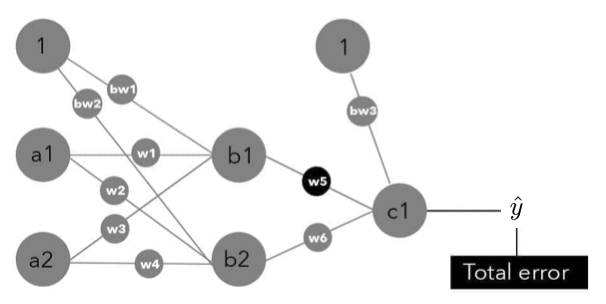
\includegraphics[width=3.5in]{figures/simple_nn_gradient.png}
    \caption{Simple Neural Network \cite{taylor2017neural}} \label{fig:gradient_nn}
\end{figure}

For this example, we will calculate the gradient of the weight $w_5$ and weight $w_1$. To calculate the gradient of weight $w_5$, we need to calculate the rate of change of the total Cross-Entropy with respect to weight $w_5$. Since this simple network only has one output neuron, denoted $c_1$, then the rate of change of total Cross-Entropy is the rate of change of the Cross-Entropy of $\hat{y}$, where $\hat{y}$ is the standardized value of output neuron $c_1$. Thus we have the gradient of weight $w_5$ as:
%
\begin{equation} \label{w5_eq1}
    \frac{\Delta \text{Tot. CE}}{\Delta w_5}= \frac{\Delta \text{CE of }\hat{y}}{\Delta w_5}
\end{equation}
%
However, weight $w_5$ does not affect the Cross-Entropy of $\hat{y}$ directly, but instead affects the net input of output neuron $c_1$, which intern affect the activation signal of $c_1$. Then and only then, output neuron $c_1$ affects the standardized value $\hat{y}$ and its Cross-Entropy. For that reason, to compute the gradient of weight $w_5$, we need to link weight $w_5$ to the Cross-Entropy of $\hat{y}$ by performing chain rule operations on the partial derivative. Apply chain rule to Equation \ref{w5_eq1} for weight $w_5$'s gradient, we have:
%
\begin{equation} \label{w5_eq2}
    \frac{\Delta \text{Tot. CE}}{\Delta w_5}
    = \frac{\Delta \text{CE of }\hat{y}}{\Delta \hat{y}}
    \times \frac{\Delta \hat{y}}{\Delta c_1}
    \times \frac{\Delta c_1}{\Delta c_1 \text{ net\_input}}
    \times \frac{\Delta c_1 \text{ net\_input}}{\Delta w_5}
\end{equation}
%
Similarly to weight $w_5$, the gradient of weight $w_1$ can also be computed using the partial derivative with the chain rule. Weight $w_1$ affects the net input of neuron $b_1$, then its activation signal. Then, Neuron $b_1$ impacts the net input of neuron $c_1$ and its activation signal. Neuron $c_1$ then affect $\hat{y}$ and its Cross-Entropy value. Notice that from neuron $c_1$ onward, the change is the same as part of weight $w_5$'s gradient formula; thus, we can expand and adapt Equation \ref{w5_eq2} to compute the gradient of weight $w_1$. The gradient of weight $w_1$ can be evaluated as follow:
%
\[
    \frac{\Delta \text{Tot. CE}}{\Delta w_1} = \frac{\Delta \text{CE of }\hat{y}}{\Delta \hat{y}} \times
    \frac{\Delta \hat{y}}{\Delta c_1} \times \frac{\Delta c_1}{\Delta c_1 \text{ netin}} \times \frac{\Delta c_1 \text{ netin}}{\Delta b_1}
    \times \frac{\Delta b_1}{\Delta b_1 \text{ netin}}
    \times \frac{\Delta b_1 \text{ netin}}{\Delta w_1}
\]
%
where "netin" stand for the net input. These examples showcase the computational process for the gradient of an in-network and an out-network weight i.e., $w_1$ and $w_5$, respectively. The same computation process for the gradient is applied to all network weights and biases, even with a more complex and higher depth network. Once the gradient is calculated for all the weights and biases, the algorithm knows how much a paticular weight or bias changes the network's total error, and thus ready to update each weight and bias accordingly.

\subsection{Backpropagation}
\textbf{Backpropagation} refer to a phase in which the algorithm using gradients of weight or bias to update their value and bring the network's total error to global minimum. Since the gradient give the slope of the loss function with respect to a weight or bias, and backpropagation update their value to approaching global minimum, thus gradient descent along with backpropagation process enable neural network to has a behavior similar to the idea of learning through the process of optimizing network's parameters. The formula to update the value of weight $w_j$ is:
%
\begin{equation} \label{backprop_func}
    \text{new } w_j = \text{old } w_j - \left( \frac{\Delta \text{Tot. CE}}{\Delta w_j} \times \eta \right)
\end{equation}
%
where old $w_j$ is the current value of weight $w_j$, $\frac{\Delta \text{Tot. CE}}{\Delta w_j}$ is the gradient of weight $w_j$, and $\eta$ refer to the algorithm's learning rate.

\textbf{Learning rate}, denoted $\eta$, is a network's hyperparameter and it determine how fast the network learn. In the updating weight function, equation \ref{backprop_func}, the learning rate directly affect the size of the step when the algorithm move toward global minimum for total error. Large leaning rate means bigger step toward minimum, thus result in faster learning, while smaller learning rate value result in slower leaning. However, a large leaning rate can also affect the network's ability to reach global minimum as it can over step and pass optimal value. Studies has shown value of a leaning rate for a multi-layer ANN should be between $10^{-16}$ and 1 with a reasonable default value of 0.01 \cite{bengio2012practical}. {\color{red} Consider put the learning rate paragraph into [section 2.3]}

As the backpropagation phase is completed, all weights and biases in the network get updated, and all four phases of the algorithm are repeated on the next batch, where the size of each batch depends on the method of gradient descent. These phases are repeated until the algorithm's total error function reaches a global minimum. At that moment, a test set will be passed through the network, and the network's total error will be returned to determine the accuracy of the algorithm.


% !TEX root = ../../username.tex
\section{Convolutional Neural Network} \label{sec:cnn}

\textbf{Convolutional Neural Network} (CNN) is a type of feedforward neural network designed to process images. A simple structure of a CNN consists of five types of layers. These layers are the input, convolutional, pooling, fully connected, and output layers. The fully connected layer is responsible for the actual classification process. Both fully connected and output layers behave the same as in a fully connected feedforward network discussed in Section \ref{sec:feedforward_nn}. A simple CNN structure for handwritten digit classification is shown in Figure \ref{fig:simple_cnn_diagram}.

\begin{figure}[!ht]
    \centering
    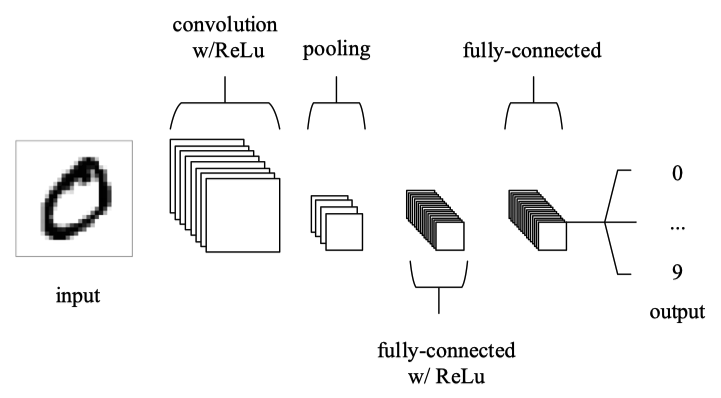
\includegraphics[width=4.5in]{figures/simple_cnn.png}
    \caption{Simple CNN structure for handwritten digit classification \cite{o2015introduction}}
    \label{fig:simple_cnn_diagram}
\end{figure}

Since an image is a 2D grid pattern data, it is possible to flatten the image and pass it through a fully connected feedforward neural network for classification directly. However, there are multiple benefits when using CNN over a standard feedforward network. The two most important benefits of CNN are spatial interaction capturing and data downsampling.

The first significant benefit is spatial interaction. \textbf{Spatial interaction} in an image refers to the connection between two or more pixel values. These connections are essential since pixels next to one another tend to describe a feature of an object, while pixels far from each other describe a different feature of the same object or a completely different object; thus, spatial interaction enhances feature extraction. On the other hand, if an image is flattened, pixels that appear close to one another will be very far away in the network, thus losing their meaning.

The second important benefit is data downsampling. \textbf{Data downsampling} refers to reducing the number of weights in the network. Consider a $64 \times 64$ RGB image, in a fully connected feedforward network, each neuron in the network will need to consider value from $64 \times 64 \times 3 = 12,288$ neurons from the previous layer. In other words, each neuron will have $12,288$ incoming connections, and the network needs to compute the gradient and do backpropagation for $12,288$ weights per neuron per network's layer. Thus, the computational and memory usage are still expensive despite the image being a low-resolution photo. Therefore, if a network could downsampling the data, it would be more efficient, have less training time, and require less computational power.

CNN is able to capture the spatial interaction and perform data downsampling using the convolutional and pooling layer before passing to a fully connected layer for classification. To further understand CNN structure, we will discuss convolutional and pooling layer functionality in detail.

\subsection{Convolutional Layer}
\textbf{Convolutional layer} is responsible for making the spatial connection and extracting features from the image. These tasks can be achieved with the use of learnable kernels. A kernel is a grid of data that has a smaller width and height but has the same depth as the input image. For example, a $64 \times 64$ RGB image will require the kernel to have the size of $x \times x \times 3$ where $x$ bounded by $2$ and $64$ inclusively. There are various types of kernels, and each type is designed to target a specific task. These tasks include blurring, sharpening, edge detection, and more. When applying the kernel to the input image, it slides from left to right and top to bottom. As it slides, the kernel's activation signal is computed by performing a scalar product of the kernel with the subregion of the image covered by it, as shown in Figure \ref{fig:kernel_op_diagram}. The kernel's activation signal represents how likely the feature -- the feature that the kernel is trying to extract -- is present at the current spatial position of the input image. The resulting grid of the kernel's activation signal is the feature map. Each kernel has an associate activation map. If multiple kernels are applied to an image, then the output feature map of these kernels will be stacked along the depth dimension.

% The kernel value are predefine for specific task. This is possible purely base on the mathematics of convolution operator. For example, a kernel with values follow the gaudience distribution, then it will give the center the kernel the highest value, and get smaller as we approach the edge of the kernel. But since the center value is effect by the value of pixels arround it, thus the sum of these make the center pixel blended in with pixels around it. Create the blurring effect.

\begin{figure}[!ht]
    \centering
    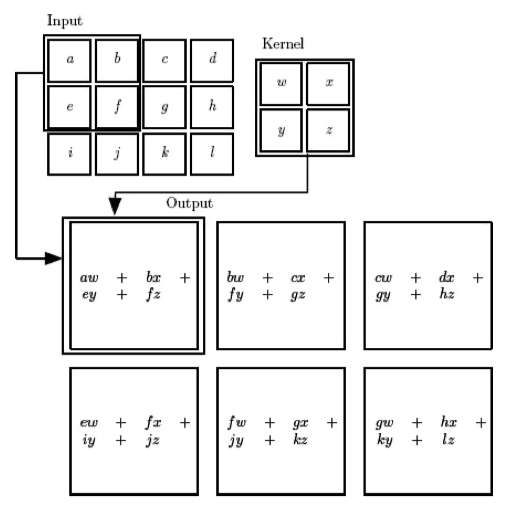
\includegraphics[width=3.5in]{figures/kernel_operation.png}
    \caption{Scalar product for a kernel's activation signal \cite{lecun2015deep}} 
    \label{fig:kernel_op_diagram}
\end{figure}
%
Notice that a kernel's width and height must be equal, and the kernel itself must be symmetric. Studies have shown that using symmetric kernels enables the algorithm to extract the inverse of a feature, thus improving the generalization for feature extraction. Additionally, since the kernel's activation signal is only based on a subregion of the image that the kernel applied to, this kernel neuron will only be connected with the neurons associated with pixels in this subregion in the network, thus reducing the number of weight in the network. The width and height of this subregion are also known as the receptive field size. Reconsider our $64 \times 64$ RGB image example, if the recaptive field is $4$, then each neuron will only have $4 \times 4 \times 3 = 48$ connections. Thus, the network will only need to compute gradient descent and do backpropagation for $48$ weights for this neuron instead of $12,288$ weights.

Other than width and height, we can also change the stride and the zero-padding to fine-tune the kernel behavior. The stride enables the kernel to slide through the image with a more significant step. That is, if the stride is 1, then the kernel will move to the left and down one pixel at a time and calculate the kernel's activation signal. Besides the stride, zero-padding also changes the convolutional behavior. The zero-padding value is the number of zero rows and columns surrounding the border of the input image. The zero-padding allows the algorithm to emphasize the border of the input image. Along with stride and zero-padding, we denoted a kernel as 
\[
    \text{kernel width} \times \text{kernel height, zero-pading size, /stride value}
\]
An the feature map size can be computed as follow:
%
\begin{equation} \label{feature_size_eq}
    \text{feature size} = \left(\frac{(\text{image size} - \text{kernel size}) + 2 \times \text{padding size}}{\text{stride}} \right) + 1
\end{equation}

\subsection{Pooling Layer}
Unlike the convolutional layer, the pooling layer only has one purpose: reducing the number of neurons in the network. The use of the pooling layer help result in fewer parameters for the network and thus require less computational power. Similar to the kernel, the pooling layer also slide through a grid of value. However, instead of sliding through the input image, the pooling layer slides through the feature map or the convoluted image to reduce the size of the feature map. There are two types of pooling layers, and they are max-pool and average-pool. As the name suggested, a max-pool layer will extract the largest activation signal in a subregion of the feature map while removing all other activation signals in the same subregion. An example of a max-pool function is shown in Figure \ref{fig:max_pool_diagram}. On the other hand, an average-pool layer takes the average value of all the activation signals in the subregion. The choice of which pooling layer to use depends on whether we care about every feature in the image equally, then the average-pool is used, or if we only care about the more prominent feature, then max-pool is used. Pooling also uses the stride to change how big of the step the pooling layer will slide through the feature map, denoted $/x$ where $x$ is stride value.
%
\begin{figure}[!ht]
    \centering
    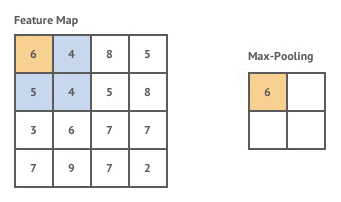
\includegraphics[width=3.5in]{figures/max_pool.png}
    \caption{$2 \times 2,\ /2$ max-pool on \cite{zeiler2014visualizing}}
    \label{fig:max_pool_diagram}
\end{figure}
%
Since pooling layer also slide throught a grid of value and output exactly one value for the subregion, thus a similar function to Equation \ref{feature_size_eq} is used to calculate the output size for pooling layer. The output size can be calculate as follow:
\[
    \text{pooling's output size} = \left(\frac{(\text{feature size} - \text{pooling size})}{\text{stride}} \right) + 1
\]

As an example, reconsider our $64 \times 64$ RGB image example, by applying a $4 \times 4, 0, \ /1$ kernel and a $2 \times 2,\ /2$ max-pool layer, the convoluted image size before passing to fully connected layer for classification is:
\[
    \text{output size} = \left[ \left( \frac{(64 - 4) + 2 \times 0}{1} + 1 \right) - 2 \right] \times \frac{1}{2} + 1 = 30 
\] 
Thus, the algorithm able to reduce from $12,288$ weights to $30 \times 30 \times 3 = 2700$ weights. In practice, it is common to have more than one kernel and one ouput apply to an input image.

% \hl{note}
% - what does NN do?
% - who came up with the idea (1-2 sentences)
% - basic des of NN architecture
% - what is limitation of NN

% Therefore, the kernel able to perform feature extraction with spatial
% connection and reduce the number of connection per neuron.

{
    \color{red}
    \subsection{Aditional term}
    \noindent TODO: \\
    \begin{itemize}
        \item overfitting problems
        \item gradient vanishing problem
        \item gaussian and uniform distribution
        \item exploding gradients
        \item batch normalzation (BN), weight normalizaiton (WN), and layer normalizaiton (LN), Local Response Normalization (LRN -- find source that LRN is not that helpful)
        \item dying ReLU
        \item input saturation
    \end{itemize}
}